\documentclass{beamer}
\usepackage[utf8]{inputenc}
\usepackage{helvet}
\usepackage{multirow}
\usepackage{graphicx}
\usepackage{amsfonts}
\usepackage{booktabs}
%\usepackage{movie15}

\useoutertheme{split}
\usecolortheme{orchid}
\usecolortheme{seahorse}

\setbeamerfont{author}{size=\footnotesize}
\setbeamerfont{date}{size=\tiny}
\setbeamerfont{title}{size=\Large, series={\bfseries}}
\setbeamerfont{subtitle}{size=\small, series=\normalfont}

\useinnertheme[shadow=true]{rounded}

\usepackage{pgf}  
\usepackage{tikz}
\logo{\pgfputat{\pgfxy(-0.2, 8.4)}{\pgfbox[right,top]{

\begin{tikzpicture}[y=0.38pt, x=0.38pt,yscale=-1, inner sep=0pt, outer sep=0pt]
\begin{scope}[cm={{1.25,0.0,0.0,-1.25,(0.0,35.4325)}}]
    \path[fill=blue,nonzero rule] (4.8090,23.2950) -- (4.8090,-0.0020) --
      (9.8590,-0.0020) -- (9.8590,23.2600) -- (15.4730,23.2600) -- (15.4730,-0.0020)
      -- (31.5390,-0.0020) -- (31.5390,23.0140) -- (37.2580,23.0140) --
      (37.2580,0.0060) -- (42.5550,0.0060) -- (42.5550,23.0140) -- (48.3440,23.0140)
      -- (48.3440,0.0060) -- (53.6410,0.0060) -- (53.6410,28.3460) --
      (26.4530,28.3460) -- (26.4530,5.1580) -- (20.6290,5.1580) -- (20.6290,28.3110)
      -- (-0.0000,28.3110) -- (-0.0000,23.2950) -- (4.8090,23.2950) -- cycle;
\end{scope}
\end{tikzpicture}
}}}


\mode<presentation>

\title{CFD Lab: Final Project}
\subtitle{3D Navier Stokes Code for Arbitrary Geometries}    %, including Free Surface}

\author{Norbert Schmidbartl, Wei Ni, Zhibin Cheng, Eva Breznik}
\institute[TUM]{Technische Universit\"{a}t M\"{u}nchen \\ Fakult\"{a}t f\"{u}r Informatik}

\date{\today}

\begin{document}

\begin{frame}
\maketitle %titlepage
\end{frame}


%\addtobeamertemplate{frametitle}{}{
%\logo{\pgfputat{\pgfxy(-0.2, 8.4)}{\pgfbox[right,top]{
%\begin{tikzpicture}[remember picture,overlay][y=0.38pt, x=0.38pt,yscale=-1, inner sep=0pt, outer sep=0pt]
%\begin{scope}[cm={{1.25,0.0,0.0,-1.25,(0.0,35.4325)}}]
%    \path[fill=blue,nonzero rule] (4.8090,23.2950) -- (4.8090,-0.0020) --
%      (9.8590,-0.0020) -- (9.8590,23.2600) -- (15.4730,23.2600) -- (15.4730,-0.0020)
%      -- (31.5390,-0.0020) -- (31.5390,23.0140) -- (37.2580,23.0140) --
%      (37.2580,0.0060) -- (42.5550,0.0060) -- (42.5550,23.0140) -- (48.3440,23.0140)
%      -- (48.3440,0.0060) -- (53.6410,0.0060) -- (53.6410,28.3460) --
%      (26.4530,28.3460) -- (26.4530,5.1580) -- (20.6290,5.1580) -- (20.6290,28.3110)
%      -- (-0.0000,28.3110) -- (-0.0000,23.2950) -- (4.8090,23.2950) -- cycle;
%\end{scope}
%\end{tikzpicture}}}}}



\begin{frame}
\frametitle{Project Topic}

\begin{columns}
\begin{column}{0.48\textwidth}
\begin{itemize}
\item 3D Navier Stokes for arbitrary geometries
\item (TO BE DETERMINED) Free Surface Flow
\end{itemize} \end{column}
\begin{column}{0.48\textwidth}
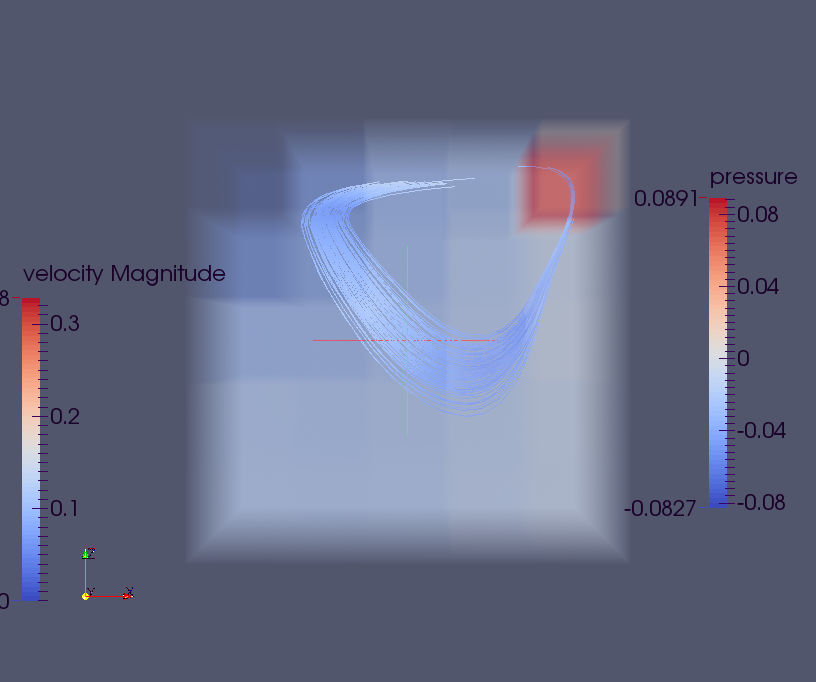
\includegraphics[height = 0.45\textheight]{simpleCavity.png}
\end{column}
\end{columns}
\end{frame}


\begin{frame}
\frametitle{Implementation}
\framesubtitle{Theory}
\scriptsize

\begin{table}[ht!]
\flushleft
\begin{tabular}{r|ccccc}
 & \bf Palabos & \bf OpenLB & \bf LBSim & \bf SailFish & \bf LB3D \\ \toprule
\bf Language &C++ (Java, Python) & C++ & C++ &Python &Fortran90 \\
\bf Visualiz.&ASCII, gif& vtk & OpenGL &numpy, vtk& XDR \\ \bottomrule
\end{tabular}
\end{table}

\end{frame}



\begin{frame}
\frametitle{Implementation}
\framesubtitle{Problems}
blablablablabblalalablbablalalalabla
\end{frame}



\begin{frame}
\frametitle{Title}
\framesubtitle{Subtitle}

\begin{itemize}
\item first
\item second
\begin{itemize}
\item second sub 1
\item second sub 2
\end{itemize}
\item own third
\end{itemize}
\end{frame}



\begin{frame}
\begin{alertblock}{{\bf Important: } Something.} 
Parameters used for the simulation: alalalalala
\end{alertblock}
\vspace{0.7cm}
\begin{columns}
\begin{column}{0.47\textwidth}
Results:
\vspace{0.4cm}
%\centering
\begin{tabular}{|c||c|}\hline
\it one & 5.217 s \\
\it two & 6.999 s \\
\it three & 5.522 s \\
\hline
\end{tabular}

\end{column}
\begin{column}{0.5\textwidth}
\flushright
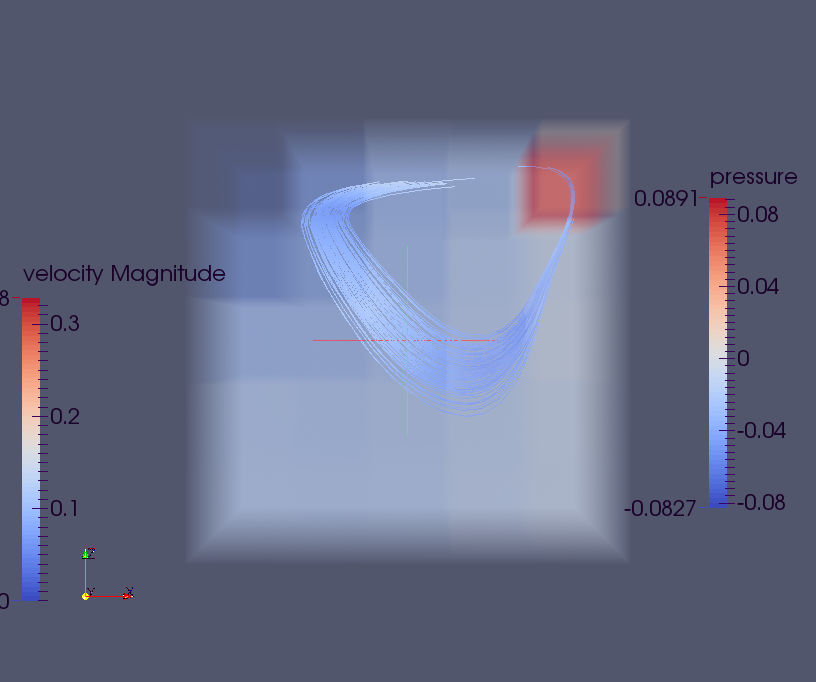
\includegraphics[height=4cm]{simpleCavity.png}
\end{column}
\end{columns}
\end{frame}


\begin{frame}
\frametitle{Some links}  %pics, movies.
{\Large \bf Palabos}\\
\begin{itemize}
\item Dam Break (free-surface flows): \\
\url{http://www.palabos.org/gallery/multi-phase-free-surface-flow/23-dam-break}
\item Volcanic Eruption \\
\url{http://www.palabos.org/gallery/incompressible-isothermal-flow/22-volcanic-eruption}
\item Rayleigh-Taylor Instability: \\
\url{http://www.palabos.org/gallery/incompressible-isothermal-flow/43-rayleigh-taylor-instability}
\end{itemize}
\end{frame}


\begin{frame}
\frametitle{Conclusion and Further Development}
have to do moro work obviously :D
\end{frame}

\end{document}
